\documentclass{beamer}
\usepackage{amsmath}
\usepackage{amssymb}
\usepackage{calc}
\usepackage{color}
\usepackage{commath}
\usepackage{fancyhdr}
\usepackage{geometry}
\usepackage{graphicx}
\usepackage{lastpage}
\usepackage{mathtools}
\usepackage{siunitx}

\begin{document}

% 
% 
% Concept of t-SNE
% 
% 
\begin{frame}
  \frametitle{Concept of t-SNE}

t-Distributed Stochastic Neighbor Embedding (t-SNE)

  \begin{itemize}
    \item a ML algorithm using for \textbf{dimensionality reduction}
    \item a variation of Stochastic Neighbor Embedding (SNE)
  \end{itemize}

Main contributions

   \begin{itemize}
    \item a \textbf{symmetrized SNE} cost function with simpler gradients
    \item the similarity computed by a \textbf{Student-t distribution} in low-dimensional space
  \end{itemize}

\end{frame}

% 
% 
% 
% Symmetric SNE
% 
% 
% 
\begin{frame}
  \frametitle{Symmetric SNE}

    \textbf{Using joint probability distribution rather than conditional probability distribution}

    the pairwise similarities in the high-dimensional space pij:
    \begin{figure}
        \centering
        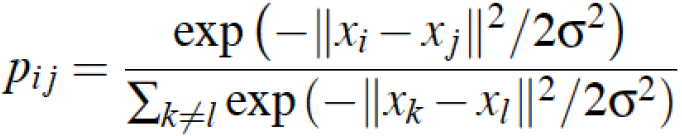
\includegraphics[height=0.1\textheight]{images/equation2.png}
    \end{figure}
    the pairwise similarities in low-dimensional map qij:
    \begin{figure}
        \centering
        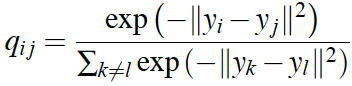
\includegraphics[height=0.1\textheight]{images/equation3.png}
    \end{figure}
    The cost function (Kullback-Leibler divergences):
    \begin{figure}
        \centering
        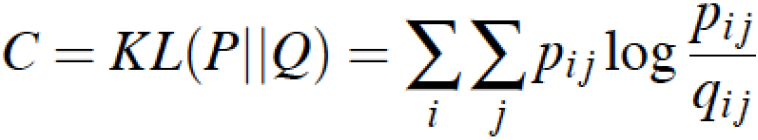
\includegraphics[height=0.1\textheight]{images/equation1.png}
    \end{figure}
    Therefore, the gradient of symmetric SNE will be optimized:
    \begin{figure}
        \centering
        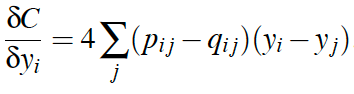
\includegraphics[height=0.1\textheight]{images/equation4.png}
    \end{figure}
\end{frame}

% 
% 
% 
% The Crowding Problem
% 
% 
% 
\begin{frame}
  \frametitle{The Crowding Problem}
  \framesubtitle{}

the area of the two-dimensional map that is available to accommodate moderately distant datapoints will \textbf{not be nearly large enough} compared with the area available to accommodate nearby datapoints.

    \begin{figure}
        \centering
        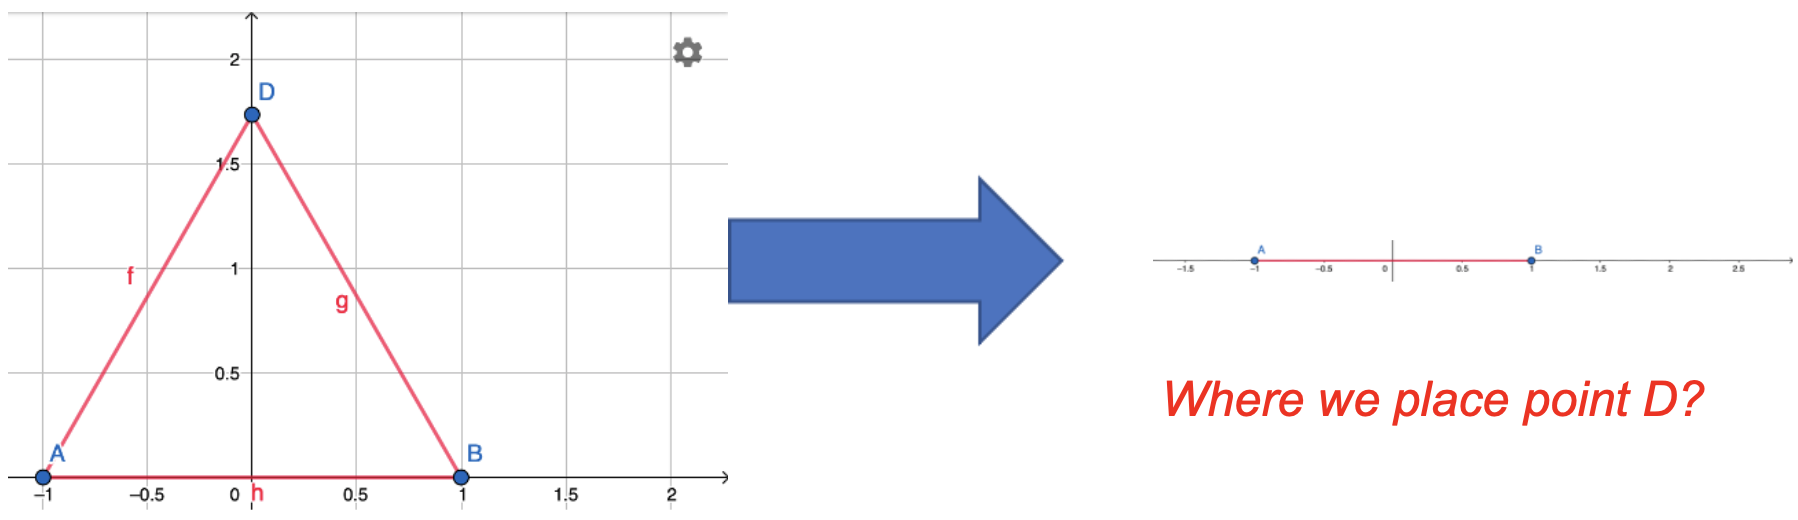
\includegraphics[height=0.3\textheight]{images/figure1.png}
    \end{figure}

\end{frame}


% 
% 
% 
% Design of t-SNE
% 
% 
%
\begin{frame}
  \frametitle{Design of t-SNE}

High-dimensional space: Gaussian distribution
    \begin{figure}
        \centering
        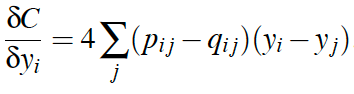
\includegraphics[height=0.1\textheight]{images/equation4.png}
    \end{figure}
Low-dimensional space: \textbf{Student t-distribution}

    \begin{figure}
        \centering
        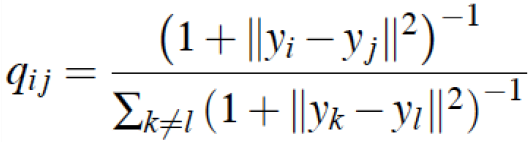
\includegraphics[height=0.1\textheight]{images/equation5.png}
    \end{figure}

The gradient of the Kullback-Leibler divergence:

    \begin{figure}
        \centering
        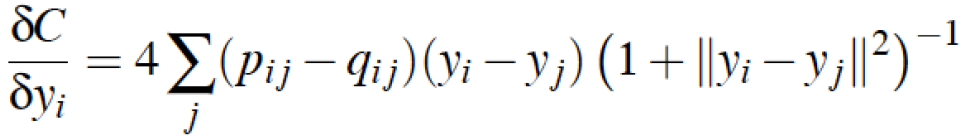
\includegraphics[height=0.1\textheight]{images/equation6.png}
    \end{figure}

\end{frame}
%
%
%
% Differences of t-dis and norm-dis
%
%
%
\begin{frame}
  \frametitle{Differences of t-dis and norm-dis}
    \begin{figure}
        \centering
        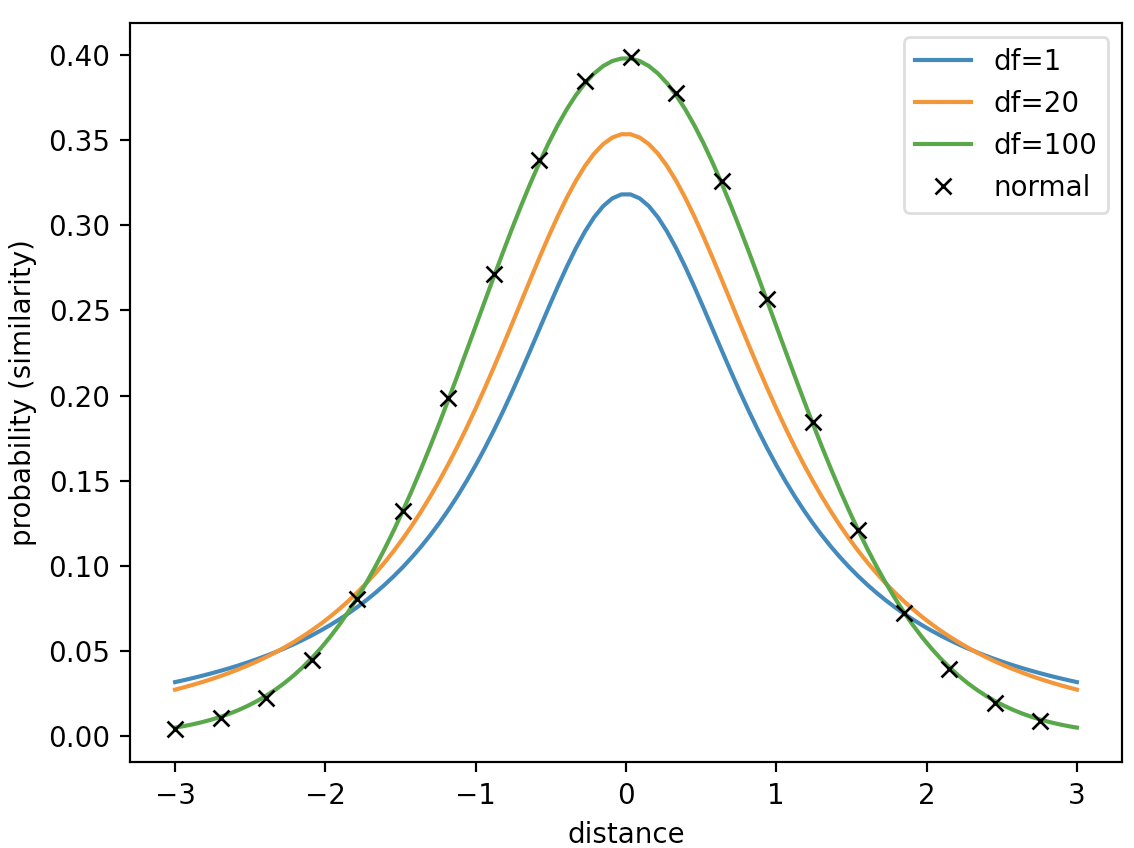
\includegraphics[height=0.6\textheight]{images/figure4.png}
    \end{figure}

\end{frame}
%
%
%
% Weakness
%
%
%
\begin{frame}
  \frametitle{Weekness of t-SNE}
    Dimensionality reduction for other purposes
    \begin{itemize}
    \item CANNOT be extrapolated to d>3 dimensions
    \end{itemize}
    Curse of intrinsic dimensionality
    \begin{itemize}
    \item LESS successful on a dataset with a high intrinsic dimensionality
    \end{itemize}
    Non-convexity of the t-SNE cost function
    \begin{itemize}
    \item the cost function is NOT convex
    \item MORE dependent on the optimization parameters
    \end{itemize}
\end{frame}



\end{document}
